\documentclass{beamer}
%\documentclass[aspectratio=169]{beamer}
%
\mode<presentation>
{
  \usetheme{default}      
  \usecolortheme{default}
  \usefonttheme{default} 
  \setbeamertemplate{navigation symbols}{}
  \setbeamertemplate{caption}[numbered]
} 

\usepackage[english]{babel}
\usepackage[utf8x]{inputenc}

\title[Classification]{Introduction to Machine Learning}
\subtitle{Lecture 3: Regression}
\author{Alexis Zubiolo\newline\texttt{alexis.zubiolo@gmail.com}}
\institute{Data Science Team Lead @ Adcash}
\date{\today}

\begin{document}

\begin{frame}
  \titlepage
\end{frame}

\begin{frame}{Before we start}
Would you be interested in \textbf{a more advanced course}? I can propose 
\begin{itemize}
	\item Machine learning \textbf{from scratch} (how to implement an ML algorithm with no library)
	\item A \textbf{more advanced version} of this course (with more theoretical technical details)
	\item \textbf{Large-scale} machine learning (distributed computing)
\end{itemize}
\end{frame}

\begin{frame}{Regression in Machine Learning}
This lecture is about \textbf{regression} in Machine learning.
\vfill
\textbf{Reminder}: In regression, the output $y$ is \textbf{continous}.
\vfill
\textbf{Example}:
\begin{itemize}
	\item \textbf{Price estimation}: $y =$ price (\textit{e.g.} 50000 BGN for a house)
	\item \textbf{Predicting the future} (\textit{e.g.} weather forecast): $y =$ temperature or amount of rain 
\end{itemize}
\end{frame}

\begin{frame}{Regression in Machine Learning: Applications}
Domains of application:
\vfill
\begin{itemize}
	\item Price estimation/prediction
\vfill
	\item Weather forecast
\vfill
	\item Production quantity estimation
\vfill
	\item Stock option price prediction
\vfill
	\item Fit statistical model to data
\vfill
	\item Physics \& chemistry
\vfill
	\item \ldots{} and others
\end{itemize}
\end{frame}
%
\begin{frame}{Linear and polynomial regression}
Purpose of regression: \textbf{approximate solutions} of \textbf{overdetermined systems}.
\vfill
\begin{figure}
\centering
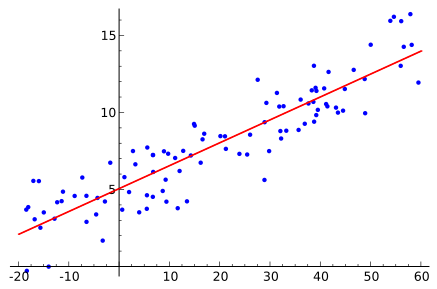
\includegraphics[width=0.70\textwidth]{images/2d_regression.png}
\end{figure}
\vfill
In this course, we will see
\begin{itemize}
	\item Linear regression
	\item Polynomial regression
\end{itemize}
\end{frame}
%
\begin{frame}
\begin{center}
\Huge{Linear regression}
\end{center}
\end{frame}
%
\begin{frame}{Linear regression}
Principal components:
\begin{itemize}
	\item Old problem (least-squares method usually credited to Carl Friedrich Gauss in 1795)
	\pause
	\item Several ways to approximate the data
	\begin{itemize}
		\item Linear model
		\item Polynomial model (remember kernels from SVMs)
		\item Fit a distribution
		\item \ldots
	\end{itemize}
	\pause
	\item Several ways to formulate the problem
	\begin{itemize}
		\item Least Squares
		\item Support Vector regression
		\item \ldots
	\end{itemize}
	\pause
	\item Several ways to solve the problem
	\begin{itemize}
		\item Closed-form expression (exact formula)
		\item Optimization
	\end{itemize}
\end{itemize}
\end{frame}



\begin{frame}{Linear regression: Toy example}

\begin{table}
\centering
\begin{tabular}{r|r|r}
living area (m$^2$) &  \textbf{\# bedrooms} & price (1000's euros) \\\hline
50 & \textbf{1} & 30\\
76 & \textbf{2} & 48\\
26 & \textbf{1} & 12\\
102 & \textbf{3} & 90\\
\pause
61 & \textbf{2} & ?
\end{tabular}
\end{table}
\pause 

\vfill
Linear model: price = \textbf{a} $\times$ area + \textbf{b} $\times$ \# bedrooms + \textbf{c}
\pause
\vfill
Problem: optimal values for \textbf{a}, \textbf{b} and \textbf{c}?
\vfill
\pause
General formulation:
\begin{equation*}
	\hat{y} = w^T x
\end{equation*}

\end{frame}

\begin{frame}{Linear regression with ordinary least-squares}
\textbf{Linear} regression: Estimate $y$ as a \textbf{linear} function of $x$:
$$ \hat{y} = w^T x$$
\vfill
\pause
\textbf{Least squares}: Penalty (loss) is a \textbf{quadratic} function
$$ \ell \left( \hat{y}, y \right) = \left( \hat{y} - y\right)^2$$
\end{frame}

\begin{frame}{Regression formulation}
2 main ways to solve the linear least-squares problem:
\begin{equation}
\label{eq:mse}
	\min_w \sum_i \left(w^T x^{(i)} - y^{(i)}\right)^2
\end{equation}

\begin{description}
	\item [Method 1: Closed-form expression]
	$$ w = \left( X^T X \right)^{-1} X^T Y $$
	It can be compuationally expensive (matrix multiplication, matrix inversion, matrix multiplication, matrix-vector multiplication)
	\item [Method 2: Numerical optimization] For example gradient descent algorithms, \ldots
\end{description}
\end{frame}

\begin{frame}
\begin{center}
\Huge{Polynomial regression}
\end{center}
\end{frame}

\begin{frame}{Polynomial regression $\approx$ Kernel trick}
Remind the kernel trick from the SVM lecture. 
\vfill
Example:
$$ x = (x_1, x_2) $$
can become 
$$ \phi(x) = (1, x_1, x_2, x_1^2, x_2^2, x_1x_2)$$
with a \textbf{second order kernel}.
\vfill
Then we can find $w$ solution of
\begin{equation}
\label{eq:mse}
	\min_w \sum_i \left(w^T \phi\left(x^{(i)}\right) - y^{(i)}\right)^2
\end{equation}
\end{frame}

\begin{frame}
\begin{center}
\Huge{Practical information}
\end{center}
\end{frame}

\begin{frame}{Variable standardization}
Variables have various magnitudes. Example:
\begin{itemize}
	\item Living area: Up to a few hundreds m$^2$
	\item Price: Up to a few 100 000s BGN (and even more)
	\item \# bedrooms: usually much smaller than 10
\end{itemize}
This can be an issue when training a regression model.
\vfill
\pause
It is possible to calculate the \textbf{standard score} z of a variable x
$$ z = \dfrac{x - \mu}{\sigma}$$
where
\begin{itemize}
	\item $\mu$ is the mean of the variable
	\item $\sigma$ is its standard deviation
\end{itemize}
\pause
\vfill
Another option: Scale between 0 and 1
$$ z = \dfrac{x - \min}{\max - \min}$$
\end{frame}

\begin{frame}{Overfitting and underfitting}
Illustration on a generated example: Try to fit the function
$$ y = f(x) = \cos \left( \dfrac{3\pi}{2} x \right) + \text{noise}$$
for $x \in [0, 1]$, with a polynomial regression
\pause
\begin{figure}
\centering
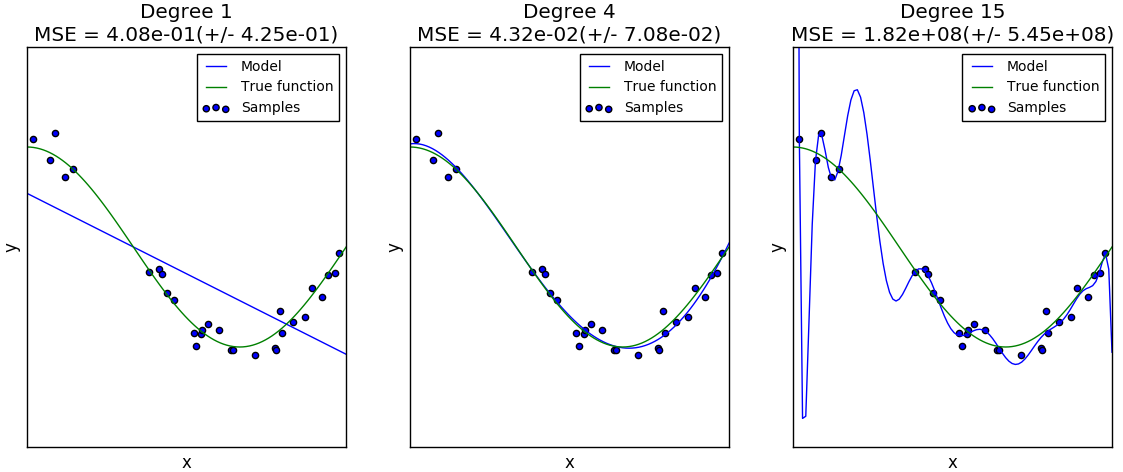
\includegraphics[width=\textwidth]{images/over_under_fitting.png}
\end{figure}
\end{frame}

\begin{frame}{Parameter selection}
As for classification models, parameter selection plays a key role in the regression performance:
\begin{itemize}
	\item Degree of the polynomial
	\item Regularization parameter
\end{itemize}
\vfill
\pause
Optimal parameters can be chosen with cross-validation over a grid:
\pause
\begin{itemize}
	\item Split the data into train/test
\pause
	\item Choose a degree $d \in \{ 1,  \dots, 20\}$
\pause
	\item Train on the train set with this degree
\pause
	\item Test the model on the test set
\end{itemize}
\vfill
\pause 
It can be done over several train/test splits.
\end{frame}

\begin{frame}{Toy example: Fitting a distribution}
Find $A$, $x_0$ and $\sigma$ such that
$$ \hat{y} = f(x) =  A e^{\dfrac{\left( x - x_0 \right)^2}{2\sigma^2}}$$
best fits the data in terms of least-square error.
\begin{figure}
\centering
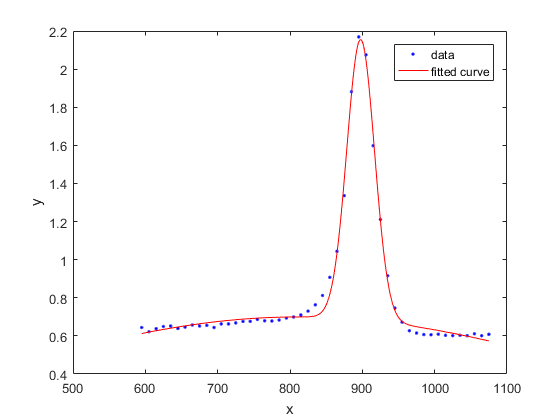
\includegraphics[width=0.75\textwidth]{images/fitted_gaussian.png}
\end{figure}
\end{frame}

\begin{frame}
\begin{center}
\Huge{Regression with SVMs}
\end{center}
\end{frame}

\begin{frame}{Alternatives to least squares}
It is possible to use a different loss function $\ell$. Remember, we had
$$ \ell \left( \hat{y}, y \right) = \left( \hat{y} - y\right)^2$$
\vfill
\pause
We can use \textbf{support vector machines for regression} (SVR):
\begin{itemize}
	\item If \textbf{within the margin} (\textit{i.e.} $ - \epsilon \leq \hat{y} - y \leq + \epsilon$) then \textbf{no penalty}
	\item linear or quadratic \textbf{penalty outside the margin}
\end{itemize}
(see flip-chart for illustration) 
\vfill
This loss function is called $\epsilon$-insensitive.
\pause
\vfill
\textbf{Note}: We can use kernels as for SVM
\end{frame}

\begin{frame}{Conclusion}
Regression: Output $y$ is a \textbf{continuous variable}.
\vfill
\pause
Several ways to \textbf{penalize errors}:
\begin{itemize}
	\item Least squares
	\item Support vector regressions
\end{itemize}
\vfill
\pause
Several ways to \textbf{model the prediction}:
\begin{itemize}
	\item Linear
	\item Quadratic
	\item Other kernel
\end{itemize}
\vfill
\pause
\textbf{Parameter selection} is important
\end{frame}


\begin{frame}
\begin{center}
\Huge{Thank you! Questions?}
\end{center}
\end{frame}

\end{document}